% This file was created with tikzplotlib v0.10.1.
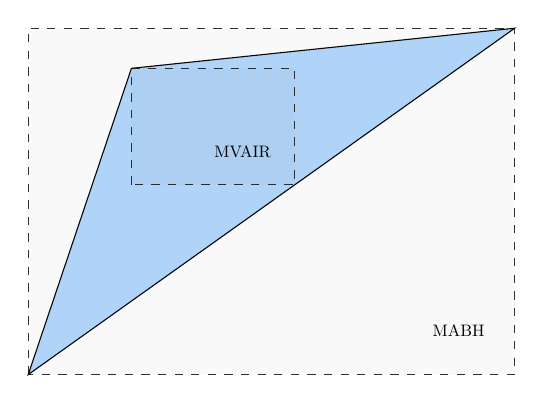
\begin{tikzpicture}

\definecolor{darkgray176}{RGB}{176,176,176}
\definecolor{dodgerblue0127255}{RGB}{0,127,255}

\begin{axis}[
hide x axis,
hide y axis,
tick align=outside,
tick pos=left,
x grid style={darkgray176},
xmin=0, xmax=1,
xtick style={color=black},
y grid style={darkgray176},
ymin=0.05, ymax=0.75,
ytick style={color=black}
]
\path [draw=black, fill=dodgerblue0127255, fill opacity=0.3]
(axis cs:0.0526315789473684,0.131578947368421)
--(axis cs:0.954022988505747,0.672413793103448)
--(axis cs:0.24390243902439,0.609756097560976)
--cycle;
\draw[draw=black,fill=gray,draw opacity=0.8,fill opacity=0.05,dashed] (axis cs:0.243902438382882,0.428048780334516) rectangle (axis cs:0.546747969914607,0.609756096574765);
\draw[draw=black,fill=gray,draw opacity=0.8,fill opacity=0.05,dashed] (axis cs:0.0526315789473684,0.131578947368421) rectangle (axis cs:0.954022988505747,0.672413793103448);
\draw (axis cs:0.45,0.48) node[
  scale=0.6,
  text=black,
  rotate=0.0
]{MVAIR};
\draw (axis cs:0.85,0.2) node[
  scale=0.6,
  text=black,
  rotate=0.0
]{MABH};
\end{axis}

\end{tikzpicture}
